% 0350(본책 66쪽) — 지름 CD(세로) 인 반원 O 에 AB, AD, BC 가 접함(□ABCD 색칠, 원문 주황), AD=6 cm, BC=10 cm. 답(넓이)은 적지 않는다. 스캔 삽화를 TikZ 로 다시 그림.
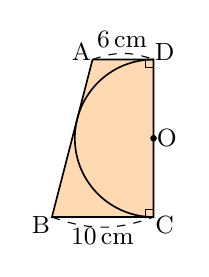
\begin{tikzpicture}[line width=0.6pt]
  \fill[orange!30] (-0.775,1.000) -- (-1.291,-1.000) -- (0.000,-1.000) -- (0.000,1.000) -- cycle;
  \draw (0.000,1.000) arc (90:270:1.000);
  \draw (-0.775,1.000) -- (-1.291,-1.000) -- (0.000,-1.000) -- (0.000,1.000) -- (-0.775,1.000);
  \fill (0.000,0.000) circle (1.2pt);
  \draw[line width=0.4pt] (-0.100,1.000) -- (-0.100,0.900) -- (0.000,0.900);
  \draw[line width=0.4pt] (-0.100,-1.000) -- (-0.100,-0.900) -- (0.000,-0.900);
  \draw[dashed, line width=0.4pt] (-0.775,1.000) to[bend left=20] (0.000,1.000);
  \node[font=\small, inner sep=1.5pt] at (-0.400,1.250) {$6\,\mathrm{cm}$};
  \draw[dashed, line width=0.4pt] (-1.291,-1.000) to[bend right=20] (0.000,-1.000);
  \node[font=\small, inner sep=1.5pt] at (-0.650,-1.250) {$10\,\mathrm{cm}$};
  \node[font=\small, inner sep=1.5pt] at (-0.915,1.100) {A};
  \node[font=\small, inner sep=1.5pt] at (0.140,1.100) {D};
  \node[font=\small, inner sep=1.5pt] at (-1.431,-1.100) {B};
  \node[font=\small, inner sep=1.5pt] at (0.140,-1.100) {C};
  \node[font=\small, inner sep=1.5pt] at (0.170,0.000) {O};
\end{tikzpicture}
